\documentclass[a4paper]{ltjsarticle}
\usepackage{luatexja}
\usepackage{luatexja-fontspec}
\usepackage{graphicx}
\usepackage{bxtexlogo}
\usepackage{tcolorbox}
\usepackage{tikz}
\usepackage{amsmath}
\usepackage{amssymb}
\usepackage{amsfonts}

\setmainfont[Ligatures=TeX]{TeXGyreTermes}
\setsansfont[Ligatures=TeX]{TeXGyreHeros}
\setmainjfont[BoldFont=HaranoAjiMincho-Bold]{HaranoAjiMincho-Regular}
\setsansjfont{HaranoAjiGothic-Medium}
\newjfontfamily\jisninety[CJKShape=JIS1990]{HaranoAjiMincho-Regular}

\tcbuselibrary{breakable, skins, theorems}

\newtcbtheorem[number within = section]{tcb}{}{enhanced, 
attach boxed title to top left = {xshift=5mm,yshift=-3mm},
boxed title style = {colframe = blue!35!black, colback = white},
coltitle = black,
colback = white,
colframe = blue!35!black,
fonttitle = \bfseries,
breakable = true,
top = 4mm
}{tcb}

\newtcbtheorem[number within = section]{axiom}{公理}{enhanced, 
attach boxed title to top left = {xshift=5mm,yshift=-3mm},
boxed title style = {colframe = blue!35!black, colback = white},
coltitle = black,
colback = white,
colframe = blue!35!black,
fonttitle = \bfseries,
breakable = true,
top = 4mm
}{axiom}
\newtcbtheorem[number within = section]{theorem}{定理}{enhanced,
attach boxed title to top left = {xshift=5mm,yshift=-3mm},
boxed title style = {colframe = blue!35!black, colback = white},
coltitle = black,
colback = white,
colframe = blue!35!black,
fonttitle = \bfseries,
breakable = true,
top = 4mm
}{theorem}
\newtcbtheorem[number within = section]{corollary}{系}{enhanced,
attach boxed title to top left = {xshift=5mm,yshift=-3mm},
boxed title style = {colframe = blue!35!black, colback = white},
coltitle = black,
colback = white,
colframe = blue!35!black,
fonttitle = \bfseries,
breakable = true,
top = 4mm
}{corollary}
\newtcbtheorem[number within = section]{proof}{証明}{enhanced,
attach boxed title to top left = {xshift=5mm,yshift=-3mm},
boxed title style = {colframe = blue!35!black, colback = white},
coltitle = black,
colback = white,
colframe = blue!35!black,
fonttitle = \bfseries,
breakable = true,
top = 4mm
}{proof}

\title{微積}

\author{kyre}
\date{\today}

%--------------------------------------------------------------------------------------------------------

\begin{document}

\section*{諸注意}
言い訳がましいが,俺は論理記号がエアプなのでイキって間違った記述をしている場合がある.説明と異なるような記述があれば,適宜指摘をお願いしたい.また,書けるところは論理記号で書いていたり,書けないところは普通に日本語を用いて書いていたりするので表記の不統一が散見されると思う.
あと普通に書いてから 1 ヶ月経過した結果かなり内容を忘れている (6/25)

\tableofcontents
\clearpage

\section{実数と数列}

\subsection{実数の連続性}

\begin{tcb}{上界と下界}{}
\begin{itemize}
\item 上界 

$\forall x \in S, x \leq a$ ならば, $a$ を $S$ の上界という.

\item 下界 

$\forall x \in S, a \leq x$ ならば,$a$ を $S$ の下界という.

\end{itemize}
\end{tcb}

また,$S \subset \mathbb{R}$ が上界をもつとき,S を上に有界であるといい,S が下界をもつときは下に有界であるという.また,これら両方をもつとき S は有界であるという.(上/下界を "持つ" だとだめっぽい?)

ここで,$S \subset \mathbb{R}$ に対して,その上界全体の集合を U(S), 下界全体の集合を L(S) と表すこととする.
このとき,U(S), L(S) を論理記号を用いて表すと
\begin{tcb}{U(S), L(S) の定義}{}
\centerline
{$
U(S) = \{a \mid \forall x \in S (x \leq a)\}
$}
\centerline
{$
L(S) = \{a \mid \forall x \in S (a \leq x)\}
$}
\end{tcb}
となる.つまり,S が 上界を持つ $\Leftrightarrow U(S) \neq \emptyset$  であるし,S が下界を持つ $\Leftrightarrow L(S) \neq \emptyset$ である.

\pagebreak

\begin{tcb}{上限と下限}{}
\begin{itemize}
\item 上限 (supremum)

$S \subset \mathbb{R}$ が上に有界である,その上界の中で最小の $x \in \mathbb{R}$ が存在するならば, $x$ を $S$ の上限であるといい,記号 $\sup S$ で表す.つまり,$U(S)$ があって $\min U(S)$ が存在するならば,それを $\sup S$ と表す.

\item 下限 (infimum)

$S \subset \mathbb{R}$ が下に有界である,その下界の中で最大の $x \in \mathbb{R}$ が存在するならば,$x$ を $S$ の下限であるといい,記号 $\inf S$ で表す.つまり $L(S)$ をもつとき,$\max L(S)$ が存在するならば,それを $\inf S$ と表す.

\end{itemize}
\end{tcb}

閉区間の集合 $[a, b]$ と開区間の集合 $(a, b)$ を考える.両者ともに区間の左端が a で,右端が b である.前者には最小値 a, 最大値 b があるが,後者には最小値も最大値も存在しない.しかし,両者はともに有界であるため,上限と下限について考えることができる.実際,$\forall x \in [a, b]$ について $ a \leq x$ であるし,$\forall x \in [a, b]$ について $x \leq b$ である.(後者に関しては,$<$ と読み替えればよい) \\ したがって,上限と下限の概念は最小値と最大値の概念よりもより広範に適用できる概念であるっぽい.

\begin{tcb}{上限と下限の性質}{}

\begin{enumerate}
\item 上に有界な集合 S について,$a = \sup S$ であることは次の条件がともに満たされることである.
\begin{itemize}
\item[(a) ] $\forall x \in S$ について $x \leq a$ である.
\item[(b) ] $a' < a$ ならば,$\exists x \in S, a' < x$ である.

つまり,$a$ より小さい上限 $a'$ を仮定しても,$a'$ より大きい $x \in S$ が存在しているよということである.
\end{itemize}
\item 下に有界な集合 S について,$a = \inf S$ であることは次の条件がともに満たされることである.
\begin{itemize}
\item[(a) ] $\forall x \in S$ について $a \leq x$ である.
\item[(b) ] $a' > a$ ならば,$\exists x \in S, a' > x$ である.

つまり $a$ より大きい下限 $a'$ を仮定しても,$a'$ より小さい $x \in S$ が存在しているよということである.
\end{itemize}
\end{enumerate}

\end{tcb}

次に,$S, T \subset \mathbb{R}, S \subseteq T$ である状況を考える.このときの $\sup S$ と $\sup T$ について,$a $ が $S$ の上界ならば,$\forall x \in S$ について $x \leq a$ だし,$\forall x \in T$ について $x \leq a$ である.よって $S$ の上界はすべて $T$ の上界でもあることがわかるから,$U(S) \subseteq U(T)$が成り立つ.同様に $\inf S$ と $\inf T$ についても考えられる.\\ \\
よって

\begin{tcb}{$S \subseteq T$ であるときの $\sup$ と $\inf$}{}
\centerline{$
S \subseteq T ならば,\sup T \geq \sup S
$}
\centerline{$
S \subseteq T ならば,\inf S \leq \inf T
$}
\end{tcb}
これらの関係は以下のように数直線上に表すとわかりやすい.

\centerline{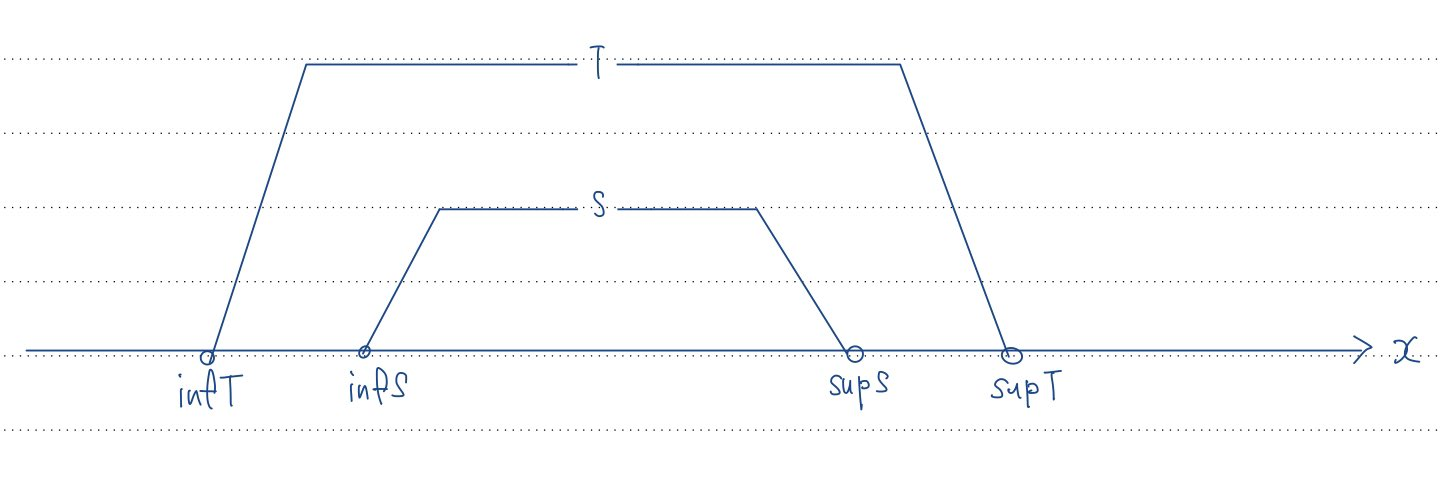
\includegraphics[width= 10cm]{./GYPtkDEb.jpg}}

\subsubsection{実数の連続性}
稠密性と連続性についてあやふやな理解をしていた.直感的に考えて $\mathbb{Q}$ にも $\mathbb{R} \setminus \mathbb{Q}$ にも数直線上で表すと隙間がある,つまり連続ではないことはわかっていたが,連続 $=$ 稠密だと思っていたのでこれらは稠密ではないと思っていた.しかし,連続性と稠密性は全く違った概念である.これらの数直線は稠密であるが,連続ではないらしい.一方,$\mathbb{R}$ は連続であり稠密である.\\
参考にした「大学教養 微分積分」ではデデキント切断とかいう名前だけはよく聞く概念による実数の連続性の定義は書かれておらず,以下の公理を認めて議論を展開するとしている.

\begin{axiom}{実数の連続性公理(Weierstrass の公理)}{}
\begin{itemize}
\item $S \subset \mathbb{R} が上に有界であるとき,\sup S が存在する.$ 
\item $S \subset \mathbb{R} が下に有界であるとき,\inf S が存在する.$
\end{itemize}

\end{axiom}

実数の連続性公理から以下が得られる.
\begin{corollary}{アルキメデスの原理}{}
\begin{itemize}
\item $ \forall a \in \mathbb{R} _ {++} (正の実数) と \forall b \in \mathbb{R} に対して,an > b となるような n \in \mathbb{N} が存在する.$

\end{itemize}
\end{corollary}
「アルキメデスの原理」という語は物理で一般に使われているが,「大学教養 微分積分」によるとこれも「アルキメデスの原理」らしい.

\begin{proof}{アルキメデスの原理の証明(写経)}{}

背理法で証明する.アルキメデスの原理の原理が成り立たないと仮定すると,$\forall n \in \mathbb{N}$ について $an \leq b$ すなわち $n \leq \frac{b}{a}$ を満たす $a \in \mathbb{R}_{++}$ と $b \in \mathbb{R}$ が存在する.よって実数の連続性公理から $\mathbb{N}$ は上に有界であり,$\sup \mathbb{N}$ が存在する.また,$\sup \mathbb{N} - 1$ は $\mathbb{N}$ の上界ではないので,$\sup \mathbb{N} - 1 < m$ となる自然数 $m$ が存在する.このとき,$\sup \mathbb{N} < m + 1$ であるから,$\sup \mathbb{N}$ より大きい自然数 $m + 1$ が存在する.このことは,$\forall n \in \mathbb{N}$ について $n \leq \sup \mathbb{N}$ であることに矛盾する.

\end{proof}


公理1.2 の不等式の両辺を n で割ると以下の系が得られる.

\begin{corollary}{}{}
任意の正の実数 a と 実数 b に対して,$a > \frac{b}{n}$ となる自然数 n が存在する.
\end{corollary}

\begin{theorem}{有理数の稠密性}{}
空集合でない開区間の中には,少なくとも一つの有理数が存在する.
\end{theorem}

\begin{proof}{有理数の稠密性の証明(写経)}{}

開区間 $(a, b) (a < b)$ を考える.$a < 0 < b$ ならば,開区間$(a, b)$ は有理数 $0$ を含む.$a < b < 0$ のとき,開区間 $(-b, -a)$ が有理数 $r$ を含む,つまり $-b < r < -a$ ならば,開区間$(a, b)$ は有理数 $-r$ を含む.よって $0 < a < b$ のときを証明すればよい.$b - a \in \mathbb{R}$ と自然数 $1$ に対して,アルキメデスの原理より,$(b - a)n > 1$ となる $n \in \mathbb{N}$ がとれる.これを変形すると $a + \frac{1}{n} < b$ であることがわかる.次に,$\frac{1}{n}, a \in \mathbb{R}$ に対して,アルキメデスの原理より $\frac{1}{n}m > a$ となる自然数 $m$ がとれる.これが成り立つような最小の$m$をとれば,$\frac{m - 1}{n} \leq a < \frac{m}{n}$ となる.このとき,$a < \frac{m}{n} = \frac{m - 1}{n} + \frac{1}{n} \leq a + \frac{1}{n} < b$ である.よって,$a < \frac{m}{n} < b$ であるから,$\frac{m}{n}$ が開区間 $(a, b)$ に属していることがわかる.(このとき,$(b-a)n > 1$ を満たす $n $を無数に取ることができる.)

\end{proof}
\begin{corollary}{}{}

$\forall \alpha \in \mathbb{R}$ と $\varepsilon \in \mathbb{R}_{++}$ に対して,$|\alpha - a| < \varepsilon$ を満たす $a \in \mathbb{Q}$ が少なくとも一つ存在する.

\end{corollary}
これは,$\alpha$ が無理数であるときに,$\alpha$ にいくらでも近い(ここガバ)有理数 a が取れることを示している.

\section{数列の収束と発散}

\begin{tcb}{極限}{}

$\forall \varepsilon \in \mathbb{R}$ に対して,ある自然数 $N$ が存在して,$n \geq N$ であるすべての自然数 $n$ について,$|a_n - \alpha| < \varepsilon$ となるとき,数列 $\{a_n\}$ は $\alpha$ に収束するという.\\
このとき,$\lim_{n \to \infty} = \alpha$ または $n \to \infty$ のとき $a_n \to \alpha$ と表す.この値 $\alpha$ を数列 $\{a_n\}$ の極限値という.$\{a_n\}$ の極限は $\alpha$ であるともいう.\\
\\
また,数列 $\{a_n\}$ が収束しないとき,$\{a_n\}$ は発散するという.\\
\\
任意の実数 $M$ に対して,ある自然数 $N$ が存在して,$n \geq N$ となる任意の自然数 $n$ について $a_n > M$ なるとき,数列 $\{a_n\}$ は正の無限大に発散する,数列$\{a_n\}$の極限は正の無限大であるといい,$\lim_{n \to \infty} = \infty$ または $n \to \infty$ のとき $a_n \to \infty$ と表す.\\
\\
任意の実数 $M$ に対して,ある自然数 $N$ が存在して,$n \geq N$ となる任意の自然数 $n$ について $a_n < M$ なるとき,数列 $\{a_n\}$ は負の無限大に発散する,数列$\{a_n\}$の極限は負の無限大であるといい,$\lim_{n \to \infty} = -\infty$ または $n \to \infty$ のとき $a_n \to -\infty$ と表す.

\end{tcb}

\begin{tcb}{$\varepsilon - N$ 論法}{}

「数列の収束について,正の実数 $\varepsilon$ が与えられたとき,$N \leq n$ となる任意の自然数 $n$ について $|a_n - \alpha| < \varepsilon$ が成り立つような $N$ を $\varepsilon$ を用いて作ることで議論する方法」を指す.このとき,$N$ は $\varepsilon$ に依存していると考えるとわかりやすい. 

\end{tcb}
手始めに,まずは $\lim_{n \to \infty} \frac{n}{n + 1} = 1$ となることを $\varepsilon - N $論法を用いて示す. 

\begin{tcb}{$\varepsilon - N$ 論法の例 1: 収束を示す}{}

取り敢えず,やりたいことは「$N < n$ である任意の自然数 $n$ について $|\frac{n}{n + 1} - 1| < \varepsilon$ が成り立つような $N$ が存在することを示す」ということだ.
\\
\\
任意の正の実数 $\varepsilon$,自然数 $m$ に対して,$|\frac{m}{m + 1} - \frac{m + 1}{m + 1}| < \varepsilon \Leftrightarrow |\frac{-1}{m + 1}| < \varepsilon \Leftrightarrow  \varepsilon  > \frac{1}{m + 1}$ である.このとき,$m + 1 \stackrel{\mathrm{def}}{=} N$ とすると $N$ 以上のすべての自然数 $n$ について,$|\frac{n}{n + 1} - 1| = \frac{1}{n + 1} \leq \frac{1}{N} < \varepsilon$ である.以上より,任意の正の実数 $\varepsilon$ に応じて,$N$ 以上の任意の $n$ について $|\frac{n}{n + 1} - 1| < \varepsilon$ が成り立つような $N$ が取れることが示された.

\end{tcb}

また,$\varepsilon - N$ 論法は数列が収束しないことを証明すること,無限大に発散することを厳密に定義することにも使える.
\begin{tcb}{$ \varepsilon - N$ 論法の例 2: 振動を示す}{}

数列 $\frac{(-1)^n}{2} = \{a_n\}$ がある実数 $\alpha$ に収束するとして,
数列 $\{a_n\}$ が $\alpha$ に収束する条件を,特に $\varepsilon = \frac{1}{2}$ のときに適用する.このとき,ある $N$ が存在して,$N \leq n$ である任意の自然数 $n$ に対して $|a_n - \alpha| < \frac{1}{2}$ となる.
\\
$n$ が奇数のときは,$a_n = \frac{-1}{2}$ であるから,$|\frac{-1}{2} - \alpha| = \frac{1}{2} + \alpha < \frac{1}{2}$ となる.このとき,$\alpha < 0$ である.
\\
$n$ が偶数のときは,$a_n = \frac{1}{2}$ であるから,$|\frac{1}{2} - \alpha| = \frac{1}{2} - \alpha < \frac{1}{2}$ となる.このとき,$\alpha > 0$ である.
これは矛盾しているため,数列 $\{a_n\}$ がいかなる実数値 $\alpha$ にも収束しない.

\end{tcb}

\begin{tcb}{$ \varepsilon - N$ 論法の例 3: 正の無限大への発散を示す}{}

数列 $\{a_n\} = 2n$ がある実数値$ \alpha$ に収束するとして,アルキメデスの原理より,$2n$ と任意の正の実数 $\varepsilon$ に対して,$\varepsilon m > 2n$ となるような自然数 $m$ が存在する. (途中)

\end{tcb}

\begin{theorem}{極限の一意性}{}

数列 $\{a_n\}$ が収束するとき,その極限値は一意に定まる.

\end{theorem}

「収束」という言葉の意味について考えると当たり前のことだが,これについても $\varepsilon - N$ 論法を用いて示すことができる.

\pagebreak

\begin{proof}{極限の一意性の証明(写経)}{}

数列$\{a_n\}$ が極限値 $\alpha$ にも $\beta$ にも収束するとして,任意の正の実数 $\varepsilon$ を考えると.$\{a_n\}$ は $\alpha$ に収束するので,ある自然数$N'$が存在して,$N' \leq n$ である任意の自然数 $n$ について $|a_n - \alpha| < \varepsilon$ となる(極限の定義そのまま)
\\
また,$\{a_n\}$ は $\beta$ にも収束するので,ある自然数 $N''$ が存在して,$N'' \leq  n$ となる任意の自然数 $n$ について,$|a_n - \beta| < \varepsilon$ となる.ここで,$N = \max \{ N', N''\}$ とする.
\\
このとき,$|\alpha - \beta| = |\alpha - a_N + a_N - \beta| \leq |\alpha - a_N| + |a_N - \beta| < \varepsilon + \varepsilon = 2\varepsilon$ である.
\\
よって,$\alpha = \beta$ であることが示された.

\end{proof}

\begin{theorem}{収束数列の有界性}{}
収束する数列 $\{a_n\}$ は有界である.
\end{theorem}

\begin{theorem}{はさみうちの原理}{}

3 つの数列 $\{a_n\}, \{b_n\}, \{c_n\}$ について,任意の自然数 $n$ に対して $a_n \leq b_n \leq c_n$ が成り立ち,$\{a_n\}$ と $\{c_n\}$ が共通の極限値 $\alpha$ に収束するとき,$\{b_n\}$ も $\alpha$ に収束する.

\end{theorem}

\begin{theorem}{部分列の極限}{}

$\{a_n\}$ を実数 $\alpha$ に収束する数列とする,このとき,$\{a_n\}$ の任意の部分列 $\{a_{n_k}\}$ も $\alpha$ に収束する.

\end{theorem}

\begin{proof}{部分列の極限の証明}
任意の正の実数 $\varepsilon$ を取る.条件より,$\lim_{n \to \infty} a_n = \alpha$

ここで,$n_k \geq N $となるような番号 $K $を取る.このとき,$K$ 以降の番号 $k$ について,$n_k \geq N$ である.このとき,$a_{n_k} = b_k$ とおくと,
$|b_k - \alpha| < \varepsilon$ が成り立つ.すなわち,任意の正の実数 $\varepsilon$ に対して,$K$ 以降の番号 $k$ について,$|b_k - \alpha| < \varepsilon$ となるような番号 $K$ をとることができた.
\end{proof}

\begin{theorem}{大小関係と極限}{}

$\{a_n\}$ を実数 $\alpha$ に収束する数列とする,このとき,実数 $a$ について $\alpha \leq a_n$ が無限個の番号 $n$ について成り立つなら,$a \leq \alpha$ である.また,実数 $b$ について $\alpha \geq b_n$ が無限個の番号 $n$ について成り立つなら,$\alpha \leq b$ である.

\end{theorem}

\pagebreak
\begin{theorem}{数列の極限の線形性}{}
\begin{itemize}
\item[1 ] $\lim_{n \to \infty} a_n b_n = \alpha \beta$
\item[2 ] $\lim_{n \to \infty} k a_n = k\alpha$
\item[3 ] $\lim_{n \to \infty} (a_n + b_n) = \alpha + \beta$
\item[4 ] $\lim_{n \to \infty} \frac{a_n}{b_n} = \frac{\alpha}{\beta}$
\end{itemize}
\end{theorem}

\begin{proof}{数列の極限の線形性 1, 2 の証明}{}

任意の正の実数 $\varepsilon$ に対して,ある自然数 $N$ が存在して,$N \leq n$ である任意の自然数 $n$ について,$|a_n - \alpha| < \varepsilon, |b_n - \beta| < \varepsilon$ が成り立つ.
\\
数列 $\{a_n\}, \{b_n\}$ は収束するため有界であるから,ある正の実数 $M$ が存在して,任意の自然数 $n$ について, $|a_n| \leq M, |b_n| \leq M$ が成り立つ.このとき,$|\alpha| \leq M, |\beta| \leq M$ も成り立つ.
性質 2 は性質 1 の $b_n$ を $k$ とおくと得られる.

\end{proof}

\begin{proof}{数列の極限の線形性 3 の証明}{}

任意の正の実数 $\varepsilon$ を取る.このとき,ある自然数 $N_1$ が存在して,$N_1 \leq n$ である任意の自然数 $n$ について,$|a_n - \alpha| < \varepsilon$ が成り立つ.また,ある自然数 $N_2$ が存在して,$N_2 \leq n$ である任意の自然数 $n$ について,$|b_n - \beta| < \varepsilon$ が成り立つ.
\\
ここで,$N = \max {N_1, N_2}$ とすれば,$N \leq n$ である任意の自然数 $n$ について,$|a_n - \alpha| < \varepsilon,|b_n - \beta| < \varepsilon$ の両方が成り立つ.したがって,$|(a_n - \alpha) + (b_n - \beta)| \leq |a_n - \alpha| + |b_n - \beta| < \varepsilon + \varepsilon = 2\varepsilon$ よって任意の正の実数 $2\varepsilon$ に対して,$N \leq n$ である任意の自然数 $n$ について $|(a_n + b_n) - (\alpha + \beta)| < 2\varepsilon$ が成り立つ.これは,数列 ${a_n + b_n}$ が $\alpha + \beta$ に収束することを示している.

\end{proof}

\section{単調数列とコーシー列}
\begin{tcb}{有界かつ単調な数列}{}

数列 $\{a_n\}$ について $a_n \leq a_{n+1} (\forall n \in \mathbb{N})$ となっているとき,数列 $\{a_n\}$ は単調に増加する,あるいは単調増加数列であるという.
また,$a_n \geq a_{n+1} (\forall n \in \mathbb{N})$ となっているとき,数列 $\{a_n\}$ は単調に減少する,あるいは単調減少数列であるという.
これらを,単調数列と呼ぶこともある.

\end{tcb}

\begin{proof}{有界かつ単調な数列の収束(写経)}{}
$\{a_n\}$ を有界かつ単調な数列であるとする.集合 $S = \{a_n | n \in \mathbb{N}\}$ は上に有界なので,実数の連続性より上限 $\alpha$ が存在する.
$\forall \varepsilon \in \mathbb{R_{++}}$ について,$\alpha - \varepsilon$ は集合 S の上界ではないので,$\alpha - \varepsilon$ < $a_N$ となる自然数 $N$ が存在する.
数列 $\{a_n\}$ は単調増加であるとしたため,$n \geq N$ であるすべての自然数について $a_N \leq a_n$ である.したがって,$\alpha - \varepsilon$ < $a_n$ である.
また,$\alpha$ は $a_n$ の上界なので $a_n \leq \alpha < \alpha + \varepsilon$ が成り立つ.よって,$\alpha - \varepsilon < a_n < \alpha + \varepsilon$ となる.
これは,$|a_n - \alpha| < \varepsilon$ と同じであり,$\varepsilon - N$論法の典型的な形になっている.
つまり,$\forall \varepsilon \in \mathbb{R_{++}}$ について,$N 以降のすべての番号 n について |a_n - \alpha| < \varepsilon$ が成り立つような番号 $N$ が取れることが示された.
ゆえに,$\{a_n\}$ が $\alpha$ に収束することが示された.
\end{proof}

\begin{tcb}{コーシー列}{}
$\forall \varepsilon \in \mathbb{R_{++}}$について ある自然数 $N$ が存在して,$k, l \geq N$ であるすべての自然数 $k, l$
について,$|a_k - a_l| < \varepsilon$ となるとき,数列 $\{a_n\}$ はコーシー列であるという.
\end{tcb}
感覚的な話をすると,項の番号が大きくなっていくとともに 2 項間の差が小さくなっていく数列がコーシー列である.

\begin{theorem}{収束数列とコーシー列(写経)}{}
数列 $\{a_n\} は収束し,\lim_{n \rightarrow \infty} a_n = \alpha$ であるとする.
$\forall\varepsilon \in \mathbb{R_{++}}$ に対して,ある自然数 $N$ が存在し,$k, l \geq N$ である \forall k, \forall l について,
$|a_k - \alpha| < \varepsilon, |a_l - \alpha| < \varepsilon$ である.
三角不等式より,$|a_k - a_l| = |a_k - \alpha + \alpha - a_l| \leq |a_k - \alpha| + |a_l - \alpha| < 2 \varepsilon$
である.$2\varepsilon$ も任意の正の実数を示すことができるため,$\{a_n\}$ のように収束する数列はコーシー列である.
\end{theorem}
三角不等式だけだからあんまり難しくないネ.

コーシーの定理については,次章で書くが,$(数列の収束)$ $\Leftrightarrow$ $(コーシー列であること)$を示す定理である.
\section{上極限と下極限}

\begin{tcb}{上極限と下極限}{}
数列 $\{a_n\}$ を有界な数列とする.$\forall n \in \mathbb{N}$ について,$k \geq n$ となる すべての自然数 $k$ について $a_k$ の上限を $\overline{a_n}$ と書く. 
同様に,$k \leq n$ となるすべての自然数 $k$ について $a_k$ の下限を $\underline{a_n}$ と書く.

これらの定義より,$\forall n$ について,$\underline{a_n} \leq a_n \leq \overline{a_n}$ が成り立つ.

$\displaystyle \lim_{n \to \infty} \overline{a_n}$ を元の数列 $\{a_n\} $の上極限と呼び,$\displaystyle \varlimsup_{n \to \infty} a_n$ または,$\displaystyle \limsup_{n \to \infty} a_n$ と書く.

$\displaystyle \lim_{n \to \infty} \underline{a_n}$ を元の数列 $\{a_n\} $の下極限と呼び,$\displaystyle \varliminf_{n \to \infty} a_n$ または,$\displaystyle \liminf_{n \to \infty} a_n$ と書く.

\end{tcb}

補題にすべきなのに定理になってるけどあんまり気にしないでください.

\begin{tcb}{コーシー列は有界である}{}
$\{a_n\}$ をコーシー列とする.数列 $\{a_n\}$ がコーシー列である条件をとくに$\varepsilon = 1$ のときに適用すると,ある番号 $N$ が存在して,$\forall k, \forall l \geq N$ について $|a_k, a_l| < 1$ となる.
特に,$\forall n \geq N$ に対して,$|a_n - a_N| < 1$ である.
三角不等式より,$|a_n| - |a_N| \leq |a_n - a_N|$であるから,$\forall n \geq$ に対して,$|a_n| < |a_N| + 1$ が成り立つ.
ここで,$N 個の実数 |a_1|, |a_2|, \ldots, |a_{N-1}|, |a_N| + 1$ の中で最大のものを $M$ とする.
このとき,$n \geq N$ の場合も,$n < N$ の場合も $|a_n| \leq M$ が成り立つ.よって,コーシー列である数列$\{a_n\}$ は有界である.

\end{tcb}

\begin{tcb}{コーシー列の上極限と下極限は一致する}{}
$\{a_n\}$をコーシー列とし,$\alpha = \displaystyle \liminf_{n \to \infty} a_n, \limsup_{n \to \infty} a_n$ とおく.コーシー列の定義から,任意の正の実数 $\varepsilon$ に対して,
ある自然数 $N_0$ が存在して,$\forall n, \forall k \geq N_0$ であるすべての自然数 $n, k$ について,$|a_n - a_k| < \varepsilon$ つまり $a_n - \varepsilon < a_k < a_n+ \varepsilon$ となる.
ここで $n \geq N_0$ である n を任意に固定して,$k \geq n $であるすべての自然数 k を考えることで,$a_n - \varepsilon \leq \underline{a_n} \leq \overline{a_n} \leq a_n + \varepsilon$

\end{tcb}

\begin{theorem}{コーシーの定理}{}
任意のコーシー列は収束する.
\end{theorem}

\end{document}
